\documentclass[]{article}
\usepackage{tikz}

%opening
\title{CSC373 Week 6}
\author{}

\begin{document}

\section{Questions}
Q: How do I generally approach answering DP Questions?\\
\begin{itemize}
	\item Try to come up with a recursive solution. Then, rewrite the algorithm to run bottom up. (ie. The base case is the same but it is used at the start of memoization instead of the deepest/last recursive call.)
\end{itemize}
Q: How do I approach test \#3 type questions? (incorrect proofs)
\begin{itemize}
	\item Make sure to follow the instructions. Many students did not give a greedy algorithm but the result of a greedy algorithm. (ex for Dijkstra: least nodes between source and destination. How is that found? BFS.)
	\item Make sure that algorithm has some meaning. There were answers that had no ending and took all edges for MST or Dijkstra.
	\item Try to keep the answer similar (lose min/max constraints). For example, it would've been sufficient to have a non-minimum spanning tree for MST and a non-minimum path tree for Dijkstra.
\end{itemize}


\section{Midterm}
\begin{itemize}
	\item Big Oh. If you had any troubles with \#1 on the midterm (especially a), make sure to review some Big Oh proofs.
	Try to use this method for fractions:
	\[\frac{n}{d} < \frac{n`}{d`}\]
	where
	\[n < n`, d > d`\]
	Basically, make the numerator larger and the denominator smaller to make the fraction larger to find a upper bound.
\end{itemize}

\section{Flow Network}
Find the max-flow of the following network. Show the residual network. Using the max-flow, what is the min cut?

%\textit{Find augmenting paths using BFS or DFS (we don't care since they are both linear). Min cut is the shortest edge on each path from A to F. Perhaps remind them that the edge weight does not relate the the edge length so we can move nodes around (or draw curvy lines for min-cut).}

\begin{figure}
	\centering
	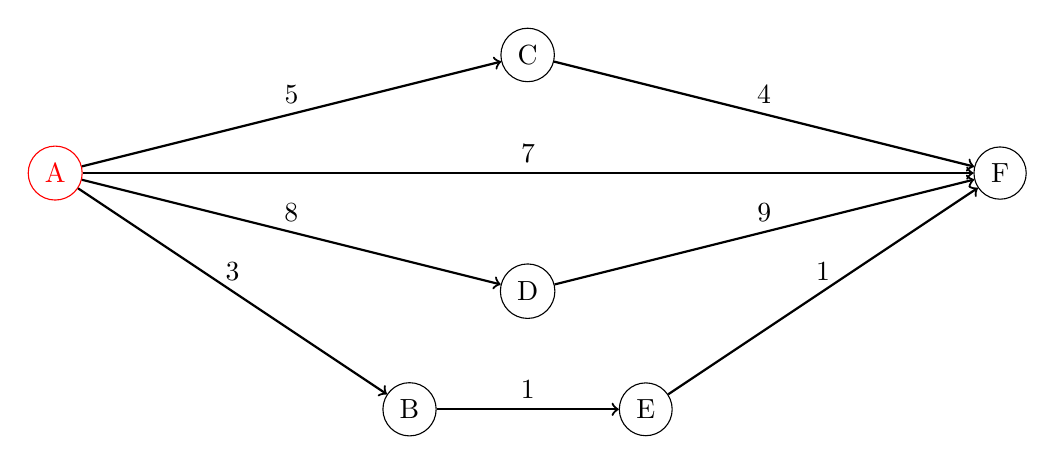
\begin{tikzpicture}
	\node[draw,circle,color=red] (A) at (-4,-1.5) {A};
	\node[draw,circle] (C) at (2,0) {C};
	\node[draw,circle] (D) at (2,-3) {D};
	\node[draw,circle] (F) at (8,-1.5) {F};
	
	\node[draw,circle] (B) at (0.5,-4.5) {B};
	\node[draw,circle] (E) at (3.5,-4.5) {E};

	
	\draw [->, thick] (A) edge node[above] {$5$} (C);
	\draw [->, thick] (A) edge node[above] {$7$} (F);
	\draw [->, thick] (A) edge node[above] {$8$} (D);
	\draw [->, thick] (A) edge node[above] {$3$} (B);
	
	\draw [->, thick] (B) edge node[above] {$1$} (E);
	
	\draw [->, thick] (C) edge node[above] {$4$} (F);
	
	\draw [->, thick] (D) edge node[above] {$9$} (F);
	
	\draw [->, thick] (E) edge node[above] {$1$} (F);
	
	%\draw [->, thick, color=red] (A) edge node[below] {$1$} (D1);
	%\draw [->, thick, color=red] (A) edge node[below] {$1$} (Dk);
	%\draw [dotted, thick] (D1) edge node[below] {} (Dk);
	
	
	\end{tikzpicture}
\end{figure}
\end{document}
